\section*{Introduction au calcul avec les fractions}

\begin{minipage}[t]{0.3\textwidth}
    Sur la figure ci-dessous :
    \begin{itemize}
        \item Colorier $\dfrac{1}{6}$ en rouge
        \item Colorier $\dfrac{4}{6}$ en bleu
        \item En déduire la valeur de $$\dfrac{1}{6}+\dfrac{4}{6}$$
    \end{itemize}
    \begin{figure}[H]
        \center
        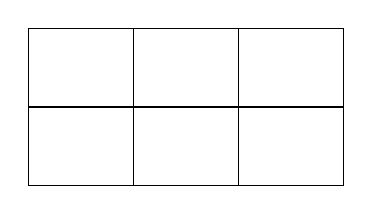
\begin{tikzpicture}[xscale=4/3]
            \draw (0,0) grid (3,2);
            \draw (0,0) rectangle (3,2);
        \end{tikzpicture}
    \end{figure}
\end{minipage}
\hfil
\vrule
\hfil
\begin{minipage}[t]{0.3\textwidth}
    Sur la figure ci-dessous :
    \begin{itemize}
        \item Colorier $\dfrac{4}{12}$ en rouge
        \item Colorier $\dfrac{5}{12}$ en bleu
        \item En déduire la valeur de $$\dfrac{4}{12}+\dfrac{5}{12}$$
    \end{itemize}
    \begin{figure}[H]
        \center
        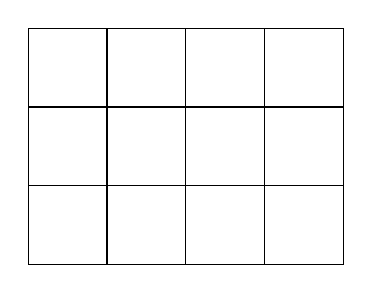
\begin{tikzpicture}
            \draw (0,0) grid (4,3);
            \draw (0,0) rectangle (4,3);
        \end{tikzpicture}
    \end{figure}
\end{minipage}
\hfil
\vrule
\hfil
\begin{minipage}[t]{0.3\textwidth}
    Sur la figure ci-dessous :
    \begin{itemize}
        \item Colorier $\dfrac{7}{15}$ en rouge
        \item Colorier $\dfrac{3}{15}$ en bleu
        \item En déduire la valeur de $$\dfrac{7}{15}+\dfrac{3}{15}$$
    \end{itemize}
    \begin{figure}[H]
        \center
        
\begin{tikzpicture}[xscale=4/5]
            \draw (0,0) grid (5,3);
            \draw (0,0) rectangle (5,3);
        \end{tikzpicture}
    \end{figure}
\end{minipage}

En déduire les calculs suivants :

\begin{multicols}{4}
    $$\dfrac{1}{5}+\dfrac{3}{5}$$

    $$\dfrac{7}{8}+\dfrac{13}{8}$$

    $$\dfrac{17}{125}+\dfrac{33}{125}$$

    $$\dfrac{743}{1524}+\dfrac{345}{1524}$$
\end{multicols}

\vfill

\begin{minipage}[t]{0.3\textwidth}
    Sur la figure ci-dessous :
    \begin{itemize}
        \item Colorier $\dfrac{1}{3}$ en rouge
        \item Colorier $\dfrac{3}{6}$ en bleu
        \item En déduire la valeur de $$\dfrac{1}{3}+\dfrac{3}{6}$$
    \end{itemize}
    \begin{figure}[H]
        \center
        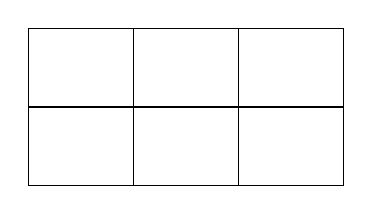
\begin{tikzpicture}[xscale=4/3]
            \draw (0,0) grid (3,2);
            \draw (0,0) rectangle (3,2);
        \end{tikzpicture}
    \end{figure}
\end{minipage}
\hfil
\vrule
\hfil
\begin{minipage}[t]{0.3\textwidth}
    Sur la figure ci-dessous :
    \begin{itemize}
        \item Colorier $\dfrac{2}{3}$ en rouge
        \item Colorier $\dfrac{3}{12}$ en bleu
        \item En déduire la valeur de $$\dfrac{2}{3}+\dfrac{3}{12}$$
    \end{itemize}
    \begin{figure}[H]
        \center
        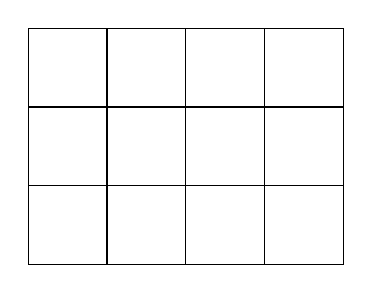
\begin{tikzpicture}
            \draw (0,0) grid (4,3);
            \draw (0,0) rectangle (4,3);
        \end{tikzpicture}
    \end{figure}
\end{minipage}
\hfil
\vrule
\hfil
\begin{minipage}[t]{0.3\textwidth}
    Sur la figure ci-dessous :
    \begin{itemize}
        \item Colorier $\dfrac{1}{3}$ en rouge
        \item Colorier $\dfrac{8}{15}$ en bleu
        \item En déduire la valeur de $$\dfrac{1}{3}+\dfrac{8}{15}$$
    \end{itemize}
    \begin{figure}[H]
        \center
        
\begin{tikzpicture}[xscale=4/5]
            \draw (0,0) grid (5,3);
            \draw (0,0) rectangle (5,3);
        \end{tikzpicture}
    \end{figure}
\end{minipage}

En déduire les calculs suivants :

\begin{multicols}{4}
    $$\dfrac{1}{5}+\dfrac{3}{35}$$

    $$\dfrac{7}{2}+\dfrac{11}{8}$$

    $$\dfrac{17}{100}+\dfrac{3}{20}$$

    $$\dfrac{111}{1000}+\dfrac{6315}{7000}$$
\end{multicols}

\newpage

%%%%%%%%%%%% PARTIE 3 %%%%%

\begin{minipage}[t]{0.3\textwidth}
    Sur la figure ci-dessous :
    \begin{itemize}
        \item Colorier $\dfrac{1}{3}$ en rouge
        \item Colorier $\dfrac{1}{2}$ en bleu
        \item En déduire la valeur de $$\dfrac{1}{3}+\dfrac{1}{2}$$
    \end{itemize}
    \begin{figure}[H]
        \center
        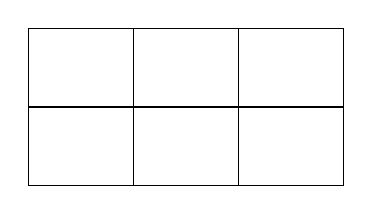
\begin{tikzpicture}[xscale=4/3]
            \draw (0,0) grid (3,2);
            \draw (0,0) rectangle (3,2);
        \end{tikzpicture}
    \end{figure}
\end{minipage}
\hfil
\vrule
\hfil
\begin{minipage}[t]{0.3\textwidth}
    Sur la figure ci-dessous :
    \begin{itemize}
        \item Colorier $\dfrac{2}{3}$ en rouge
        \item Colorier $\dfrac{1}{4}$ en bleu
        \item En déduire la valeur de $$\dfrac{2}{3}+\dfrac{1}{4}$$
    \end{itemize}
    \begin{figure}[H]
        \center
        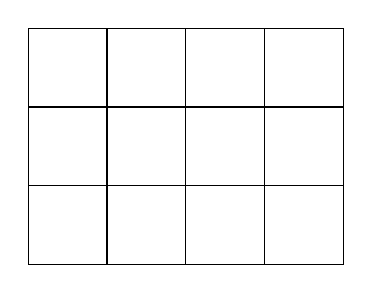
\begin{tikzpicture}
            \draw (0,0) grid (4,3);
            \draw (0,0) rectangle (4,3);
        \end{tikzpicture}
    \end{figure}
\end{minipage}
\hfil
\vrule
\hfil
\begin{minipage}[t]{0.3\textwidth}
    Sur la figure ci-dessous :
    \begin{itemize}
        \item Colorier $\dfrac{2}{3}$ en rouge
        \item Colorier $\dfrac{2}{5}$ en bleu
        \item En déduire la valeur de $$\dfrac{2}{3}+\dfrac{2}{5}$$
    \end{itemize}
    \begin{figure}[H]
        \center
        
\begin{tikzpicture}[xscale=4/5]
            \draw (0,0) grid (5,3);
            \draw (0,0) rectangle (5,3);
        \end{tikzpicture}
    \end{figure}
\end{minipage}

En déduire les calculs suivants :

\begin{multicols}{4}
    $$\dfrac{1}{7}+\dfrac{2}{3}$$

    $$\dfrac{1}{2}+\dfrac{4}{5}$$

    $$\dfrac{7}{2}+\dfrac{5}{3}$$

    $$\dfrac{17}{100}+\dfrac{5}{3}$$
\end{multicols}